\documentclass[a4paper, 12pt]{report}

\usepackage[utf8]{inputenc}
\usepackage[T1]{fontenc}
\usepackage{lmodern}
\usepackage[ngerman]{babel}
\usepackage[margin=3.0cm,top=4cm]{geometry}
\usepackage[]{graphicx}

\usepackage{array}
\usepackage{lastpage}
\usepackage{blindtext} 
\usepackage{amsmath} 
\usepackage{nicefrac}
\usepackage{float}


\newcolumntype{L}[1]{>{\raggedright\let\newline\\\arraybackslash\hspace{0pt}}m{#1}}
\newcolumntype{C}[1]{>{\centering\let\newline\\\arraybackslash\hspace{0pt}}m{#1}}
\newcolumntype{R}[1]{>{\raggedleft\let\newline\\\arraybackslash\hspace{0pt}}m{#1}}


\usepackage{sectsty}
\sectionfont{\fontsize{12}{15}\selectfont}

\renewcommand{\familydefault}{\sfdefault}

\usepackage{fancyhdr}

\pagestyle{fancy}
\fancyhf{}
\fancyhead[L]{Tiefpass-Bandsperre-Transformation}
\fancyhead[R]{Stefan Urban}
\fancyfoot[R]{Seite \thepage\ von \pageref{LastPage}}
\renewcommand{\headrulewidth}{0.4pt}

%\addtolength{\parskip}{2mm}
\setlength{\parindent}{0pt}


\begin{document}

\section*{1. Mittenfrequenz berechnen}
	\[ f_m = \sqrt{f_{+p} \cdot f_{-p}} \]
	
\section*{2. Normierte Bandbreite B und Transformationskonstante k berechnen}
	\[ k = \frac{1}{B} = \frac{f_m}{f_{+p} - f_{-p}} \]
	
\section*{3. Abstand der Sperrfrequenzen von der Mittenfrequenz prüfen und anspassen}
	\[ \frac{f_{+s}}{f_m} \stackrel{!}{=} \frac{f_m}{f_{-s}} \]
	
\section*{4. Normierte Tiefpass-Sperrfrequenz berechnen}
	\[ \Omega_{sTP} = \frac{f_{+p} - f_{-p}}{f_{+s} - f_{-s}} \]
	
\section*{5. Aufwandsabschätzung}
	\begin{minipage}[t]{0.33\textwidth} 
			\[  \frac{d}{c} = \sqrt{\frac{10^{a_s / 10dB} - 1}{10^{a_p / 10dB} - 1}}  \]
	\end{minipage} 
	\begin{minipage}[t]{0.33\textwidth} 
			\begin{center}
			Tschebyscheff
			\end{center}
			\[ n \ge \frac{\cosh^{-1}{\left(\frac{d}{c}\right)}}{\cosh^{-1}{\left(\Omega_{sTP}\right)}} \]
	\end{minipage}
	\begin{minipage}[t]{0.33\textwidth} 
			\begin{center}
			Butterworth
			\end{center}
			\[ n \ge \frac{\log{\left(\frac{d}{c}\right)}}{\log{\left(\Omega_{sTP}\right)}} \]
	\end{minipage}
	
\section*{6. Pole des Referenztiefpasses bestimmen}
	Butterworth Polwinkel berechnen
	
	\begin{minipage}[t]{0.33\textwidth}
		\vspace{-0.5cm}
		\[ \Omega_{xBW} = \frac{1}{\sqrt[2n]{10^{a_p / 10dB} - 1}} \]
	\end{minipage}
	\begin{minipage}[t]{0.66\textwidth}
		\[ \Theta_{BW} = 180^{\circ} \cdot \frac{2k-1}{2n}  \qquad  k = 1, 2, ... n \]
	\end{minipage}
	
	\vspace{0.5cm}
	
	Tschebyscheff Polfrequenzen und -winkel berechnen

	\begin{minipage}[t]{0.33\textwidth}
			\[ c = \sqrt{10^{a_p / 10 dB} - 1} \]
	\end{minipage}
	\begin{minipage}[t]{0.33\textwidth}
			\vspace{0.4cm}
			\[ \ln{\alpha} = \sinh^{-1}{\frac{1}{c}} \]
	\end{minipage}
	\begin{minipage}[t]{0.33\textwidth}
			\[ R_i = \sinh{\frac{\ln{\alpha}}{n}} \]
			\[ R_a = \cosh{\frac{\ln{\alpha}}{n}} \]
	\end{minipage}
	
	\begin{minipage}[t]{0.6\textwidth}
		\[ \Omega_{xT} = \sqrt{(R_i \cdot \sin{\Theta_{BW}})^2 + (R_a \cdot \cos{\Theta_{BW}})^2} \]
	\end{minipage}
	
	\vspace{0.5cm}
	
	\begin{minipage}[t]{0.6\textwidth}
		\[ Q_T = \frac{1}{2} \cdot \sqrt{1 + \left(\frac{R_a / R_i}{\tan{\Theta_{BW}}}\right)^2} \]
	\end{minipage}
	\begin{minipage}[t]{0.4\textwidth}
		\[ \Theta_T = \sin^{-1}{\frac{1}{2 \cdot Q_T}} \]
	\end{minipage}
	

\clearpage

\section*{7. Pole der Bandsperre berechnen}

	Tiefpass ist normiert auf Durchlassgrenzfrequenz, Bandsperre ist normiert auf Mittenfrequenz.
	
	\begin{minipage}[t]{0.5\textwidth}
		\vspace{-0.5cm}
		\begin{align*}
			P_{BS} &= \frac{1}{2k \cdot P_{TP}} \pm \sqrt{\left( \frac{1}{2k \cdot P_{TP}} \right)^2 - 1} &\\
			&= \frac{B}{2 \cdot P_{TP}} \pm \sqrt{\left( \frac{B}{2 \cdot P_{TP}} \right)^2 - 1} &
		\end{align*}
	\end{minipage}
	\begin{minipage}[t]{0.5\textwidth}
		\vspace{-0.5cm}
		\begin{align*}
			\frac{1}{P_{TP}} &= k \cdot \left(P_{BS} + \frac{1}{P_{BS}}\right) &\\
			&= \frac{P^2_{BS} + 1}{B \cdot P_{BS}} &
		\end{align*}
	\end{minipage}
	
	\vspace{0.4cm}
	
	Hinweis: Taschenrechner kann keine Wurzel aus einer komplexen Zahl ziehen.
	
	\begin{figure}[H]
		\centering 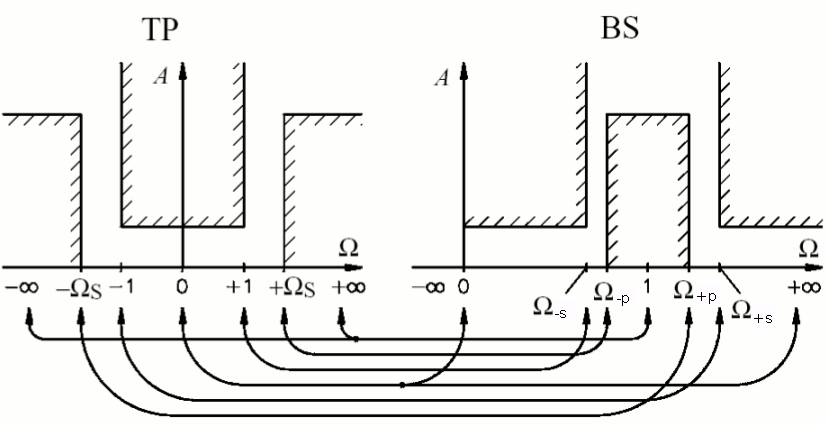
\includegraphics[width=0.9\textwidth]{images/tiefpass-bandsperre-transformation.png}
		\caption{Geometrisch-symmetrische Transformation: TP $ \Leftrightarrow $ BS}
	\end{figure}
	
	\begin{center}
		\begin{tabular}{|C{3cm}|C{3cm}|}
		\hline \textbf{Tiefpass} & \textbf{Bandsperre} \\ 
		\hline $ 0 $ & $ 1 $ \\ 
		\hline $ \pm 1 $ & $ \Omega_{\pm p} $ \\ 
		\hline $ \pm \Omega_s $ & $ \Omega_{\pm s} $ \\ 
		\hline 
		\end{tabular} 
	\end{center}
	
	\underline{Mathematik-Exkurs:} Komplexe Zahl unter der Wurzel:
	
	\[ \underline{z} = r \cdot e^{j\varphi} \qquad \sqrt[n]{\underline{z}} = \sqrt[n]{r} \cdot e^{\frac{\varphi + 2\pi k}{n}} \qquad k = 0, 1, ... (n-1) \]
	
	\begin{minipage}[t]{0.4\textwidth}
		\vspace{0.17cm}
		\begin{flushright}
			z.B. für $ n = 2 $
		\end{flushright}
	\end{minipage}
	\begin{minipage}[t]{0.6\textwidth}
		\vspace{-0.5cm}
		\begin{flalign*}
			\qquad z_1 &= \sqrt{r} \cdot e^{j\varphi} &\\
			z_2 &= \sqrt{r} \cdot e^{j \cdot ( \varphi + 180^{\circ} ) } &
		\end{flalign*}
	\end{minipage}
	
\section*{8. Nullstellen der Bandsperre}
	Eine Bandsperre besitzt $ n_{TP} $ Nullstellen bei $ p = j $ und $ n_{TP} $ Nullstellen bei $ p = -j $.

\end{document}
